\documentclass[10pt]{beamer}
\usetheme{Warsaw}
\usepackage[MeX]{polski}
\usepackage[utf8]{inputenc}
\usepackage[polish]{babel}
\usepackage{hyperref}
\usepackage{color}

\theoremstyle{definition}
\newtheorem{definicja}{Definicja}

\title[Clustering danych giełdowych]{ 
  Hurtownie Danych i Data Mining\\
  \small{Prezentacja prac nad projektem}\\
  	Wpływ wydarzeń politycznych, ekonomicznych i naturalnych
  	na kształtowanie się cen akcji na rynku polskim
 }
\author{Tomasz Kupczyk, Patryk Obara, Karol Stosiek}
\institute{Instytut Informatyki Uniwersytetu Wrocławskiego}
\date{11 maja 2010}

\begin{document}

\begin{frame}
  \titlepage
\end{frame}

\begin{frame}{Plan prezentacji}
\tableofcontents
\end{frame}

\section{Definicja problemu}

\frame{
  \begin{definicja}
  Obserwacje wahań kursów akcji pojedynczych spółek na giełdach papierów wartościowych wykazują pewną korelację z wydarzeniami politycznymi, ekonomicznymi i naturalnymi. Celem projektu jest próba zgrupowania tych spółek giełdowych w grupy wykazujące podobne zachowanie i zbadanie, które z tych grup są podatne na wydarzenia historyczne z uwzględnieniem kategorii tych wydarzeń. 
  \end{definicja}
}

\section{Dane}

\frame{
\begin{itemize}
  \item Dane spółek wyłącznie z GPW w Warszawie.
  \item Na GPW notowanych jest około 350 spółek.
  \item Nasze dane obejmują 186 spółek.
  \item Okres czasu: każda ze 186 wybranych przez nas spółek była notowana w okresie od 09-02-2009 do 16-04-2010 (300 dni, bez "dziur"). 
  \item Jest to najdłuższy okres, w którym każda ze 186 wybranych spółek była notowana na GPW, jaki udało nam się znaleźć.
  \item Dane pochodzą z serwisu www.bossa.pl.
\end{itemize}
}

\section{Metody}

\frame{
\begin{itemize}
  \item K-means.
  \item Hierarchical clustering.
  \item Self-Organizing maps.
\end{itemize}
}

\frame{
 \frametitle{Self-Organizing maps}
\begin{center}
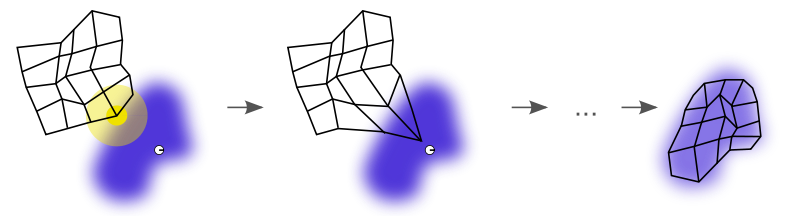
\includegraphics[scale=0.4]{som.png} 
\end{center}
}

\section{Wyniki}

\frame{
 \frametitle{K-means}
 Ilość iteracji: 100;
 Ilość grup: 5, 10, 20;
 Miara odległości: euklidesowa.
 \begin{itemize}
 \item Dla parametru k=20 daje coraz rozsądniejszy podział na grupy spółek zachowujących się podobnie (ca. 10 grup spółek ma sens)
 \item Dla wektorów cen daje bardzo liczne grupy, ale spółki zachowują się podobnie w obrębie grup;
 \item Dla wektorów różnic cen daje w zasadzie jedną bardzo liczną grupę spółek, co uniemożliwia sensowną analizę;
 \item W obydwu przypadkach przynajmniej połowa otrzymanych grup to grupy zawierające niewielką ilość spółek (1,2,3).
 \end{itemize}
}

\frame{
 \frametitle{Hierarchical clustering}
 \begin{itemize}
 \item TODO
 \end{itemize}
}

\frame{
 \frametitle{Self-Organizing maps}
 \begin{itemize}
 \item TODO
 \end{itemize}
}

\frame{
 \frametitle{Wydarzenia historyczne}
 \begin{itemize}
 \item TODO
 \end{itemize}
}

\section{Plany na przyszłość}
\frame{
}

\section{Używane narzędzia}

\frame{
\href{http://bonsai.ims.u-tokyo.ac.jp/~mdehoon/software/cluster/software.htm}{Pycluster}

\begin{center}

\includegraphics[scale=0.25]{python-powered.png} 
\end{center}
}

\frame{
\href{http://www.gnuplot.info/}{gnuplot}

\begin{center}
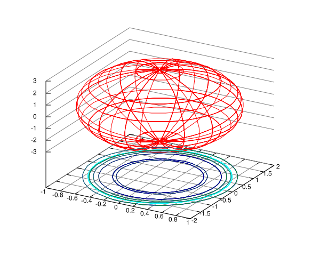
\includegraphics[scale=0.5]{gnuplot_ellipsoid.png} 
\end{center}
}

\frame{
\begin{center}
Dziękujemy za uwagę.
\end{center}
}
\end{document}
